\chapter{Axisymmetric model for the southern jet}
\label{chapter8}

%\textbf{(b)} Zoom-in of the top rectangular region in a) showing the bright knots in the northern jet. Contours are at 1.5, 2.7, 3.7, 5.1, 6.3, 7.5, 8.8, 10, 21, 37, 51, 72, 90, 103, 154, 311, and 466 mJy arcsec$^{-2}$. \textbf{(c)} Zoom-in of the bottom rectangular region in a) showing the bright knots in the southern jet. Contours are at 1.5, 2.0, 2.2, 2.7, 3.7, 5.1, 5.5, 6.0, 6.3, 6.8, 7.5, 8.8, 10, 21, 37, 51,  72, 90, 103, 154, 311, and 466 mJy arcsec$^{-2}$.

In chapter~\ref{chapter5} I presented a detailed study of the Hydra A northern jet focusing on two bright knots and the oscillation in jet radius of the central 10~kpc jet stream. Here, I consider the implications of the knot structures in the southern jet. In the southern jet, there are \emph{four} knots, compared to just two in the northern jet. The knots are at 2.5, 3.9, 5.4, and 6.7 kpc from the core. The four bright knots and the locations of the associated reconfinement shocks are shown in Fig.~\ref{southern}.

The reality of the knot at 2.5 kpc is debatable because of the low surface brightness there and the gap in surface brightness between that feature and the core. For the following, I assume that it is in fact a knot formed due to a reconfinement shock. The main reason for this assumption is that the location of the knot fits into the sequence of regular shock spacing as predicted for a sequence of reconfinement shocks.

The southern jet is not as amenable to hydrodynamic modelling as the northern jet. First, there is the gap in the surface brightness data between the core and the first knot. Second, the jet stream in the inner 10 kpc of the southern jet is more curved than that of the northern jet, stretching the validity of the axis-symmetric approximation, as used in chapter~\ref{chapter5}. Regarding this point, I note that, at least in projection, the second, third, and fourth knots are fairly well aligned along a straight line. Third, there has been no determination of the jet radius versus distance from the core, as there has been for the northern jet. Hence, all in all, the southern jet data do not provide as good a basis for parameter estimation. Nevertheless, it is of interest to apply the previous approach to the southern jet in order to see what similarities and difference in parameters one obtains. 

The results presented below reinforce the velocity estimates for the northern jet. There is one interesting difference in that the optimal model has an initial overpressure ratio of unity. 

\begin{figure}
\centering
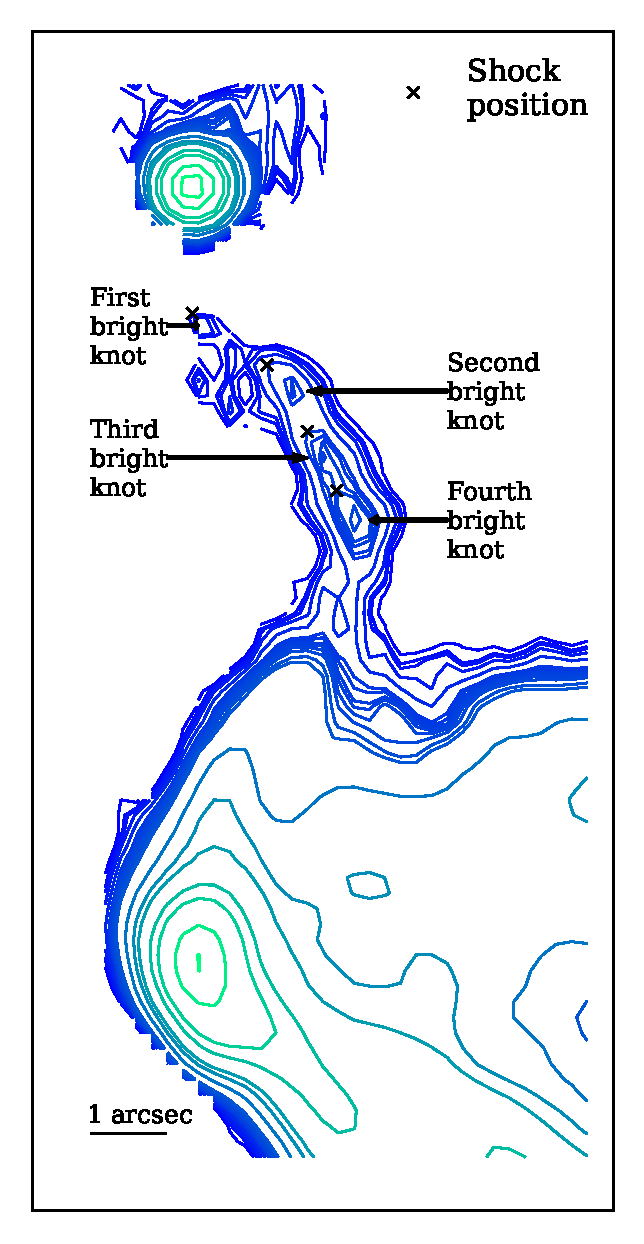
\includegraphics[width=5cm]{southern.eps}
\caption{ Radio intensity map of the central 20~kpc region of the Hydra~A southern jet at 4.635 GHz. Contour levels are at 1.5, 2.0, 2.2, 2.7, 3.7, 5.1, 5.5, 6.0, 6.3, 6.8, 7.5, 8.8, 10, 21, 37, 51,  72, 90, 103, 154, 311, and 466 mJy arcsec$^{-2}$. Four bright knots are marked by arrows. The location of the reconfinement shocks which we interpret as the cause of bright knots are marked by $\times$s. }
\label{southern}
\end{figure}

Guided by the models for the northern jet, I perform a parameter study for the southern jet on the basis of the same proposition that the four bright knots in the southern jet (see Fig.~\ref{taylor}) are the consequence of four consecutive biconical shocks at 2.5, 3.9, 5.4, and 6.7 kpc. As I discussed earlier, because of the lack of observational data for the radius profile of the jet within 5 kpc from the core, I only consider the shock positions of this jet.

\subsection{Parametric study for the southern jet}\label{s:param_study}
\begin{figure*}[ht!]
\includegraphics[width=\textwidth]{sps.eps}
\caption{Shock positions, marked by points, for different jet velocities (bottom $x$-axis) and different pressure ratios (top $x$-axis). The horizontal solid lines represent the observed shock locations of the southern jet. The models presented here are different from the best fit model for Hydra A northern jet (Ciii, in chapter~\ref{chapter5}), in either the jet velocity or, in the over-pressure ratio. Note that the values on the horizontal axes representing the jet over-pressure ratio and the jet velocity are ordered to show all combinations of parameters tested. A visual comparison of the shock locations between the simulations and the observations shows that the best fit model of the southern jet is the model for which $p_{\rm jet}/p_{\rm a}=1$, and $\beta = 0.8$.  }
\label{p_s_s}
\end{figure*}

%The blue dashed lines represent the shock location for the model Ciii of the northern jet. The green solid line represent the observed shock locations of the southern jet. Panel (a) and (b) comprises models deviated from the model Ciii in the jet velocity and the pressure ratio respectively. Panel (c) comprises models with pressure equilibrium jet and with different jet velocities. A visual comparison of the shock locations between the simulations and the observations shows that the best fit model for the southern jet is with $p_\mathrm{jet}/p_\mathrm{a} = 1$, and $\beta = 0.8$.

\begin{figure}[ht!]
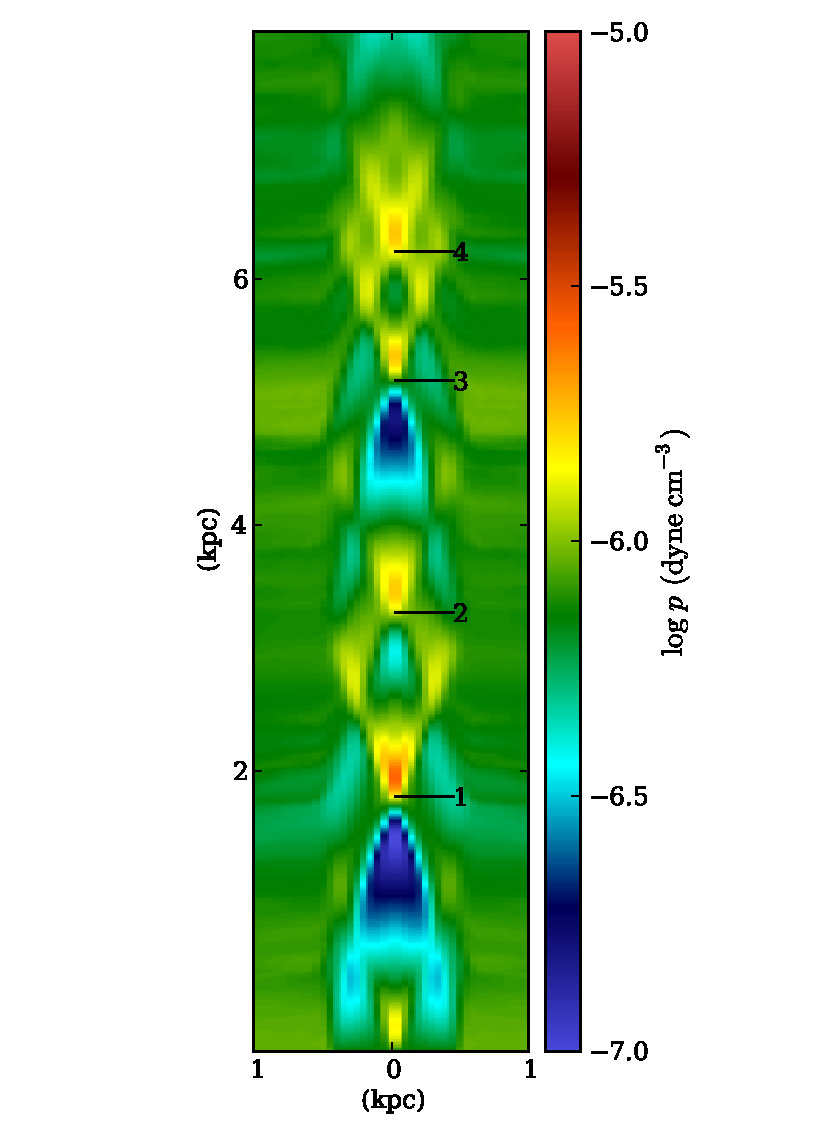
\includegraphics[width=\linewidth]{sbm.eps}
\caption{Logarithmic pressure image of the best fit model for the southern jet (run Ev). The image shows the four biconical shocks along the jet marked by 1, 2, 3 and 4.}
\label{m_s_p}
\end{figure}


\begin{table*}
%\begin{sidewaystable}
\caption{Simulation parameters. In all simulations, $P_{\rm{jet}}=10^{45} \rm \ erg \ s^{-1}$.}
\centering
\begin{tabular}{l * {8}{c}}
\hline \hline
Simulation  & $p_{\rm{jet}}/p_{\rm{a}}$ & $\beta$ & $\chi$ & $\eta$ & $\phi$ (rad cm$^{-2}$) & $\Psi_{6\rm{cm}}$ (rad) & $\Psi_{20\rm{cm}}$ (rad) \\
\hline
    %%%%%%%%%% 		set A 	%%%%%%%%%%%%%%%
	\multicolumn{8}{c}{Set E, $r_{\rm{jet}}=0.10 \rm \ kpc$} \\ 
	\hline
  	Ei      & 5    & 0.95 & 0.57    & 3.18$\times10^{-5}$   & 1.61$\times10^{-5}$   & 5.80$\times10^{-4}$   & 6.45$\times10^{-3}$   \\
	Eii     & 5    & 0.96 & 0.15    & 8.33$\times10^{-6}$   & 4.22$\times10^{-6}$   & 1.52$\times10^{-4}$   & 1.69$\times10^{-3}$   \\
	Eiii	& 2   & 0.80 & 35.63    & 7.97$\times10^{-4}$   & 4.04$\times10^{-4}$   & 1.45$\times10^{-2}$   & 1.61$\times10^{-1}$ \\
	Eiv	& 1  & 0.75   & 113.85 & 1.27$\times10^{-3}$   & 6.45$\times10^{-4}$ & 2.32$\times10^{-2}$ & 2.58$\times10^{-1}$ \\
	Ev    & 1  &  0.80  & 73.77   &  8.25$\times10^{-4}$   & 4.18$\times10^{-4}$   & 1.50$\times10^{-2}$   & 1.67$\times10^{-1}$   \\
	Evi      & 1    & 0.85 &  44.66  & 4.99$\times10^{-4}$   & 2.53$\times10^{-4}$   & 9.10$\times10^{-3}$   & 1.01$\times10^{-1}$   \\
		\hline
\end{tabular}
\label{t:sim_par_s}
%\end{sidewaystable}
\end{table*}

For the parameter space study of the southern jet, I performed a series of axis-symmetric relativistic hydrodynamic simulations with the same general setup as for the parameter study of the northern jet (chapter \ref{chapter5}). For the southern jet, I fix the jet power and jet radius to the values of the best-fit model for the northern jet at $P_\mathrm{jet} = 10^{45}$ erg s$^{-1}$ and $r_\mathrm{jet}=100$pc, respectively, and vary only the two other independent jet parameters, the jet velocity and the pressure ratio between the jet and the ambient medium. Because the spacing of the shocks in the southern jet is smaller than that in the northern jet, I explored slightly higher ranges of the jet velocity for a given value of $p_\mathrm{jet}/p_\mathrm{a}$. I  also performed runs with pressure ratios $p_\mathrm{jet}/p_\mathrm{a}=2$ and 1. Simulation parameters for the different models are presented in Table~\ref{t:sim_par_s}.

The parameter $\chi$, which is determined by the other jet parameters through Eqn.~\ref{chi2} becomes negative for jet velocities greater than 0.96, so that this represents the maximum possible jet velocity. I therefore explored values of the pressure ratio $p_\mathrm{jet}/p_\mathrm{a} = 2 \rm  \ and \ 1$, keeping the jet velocity fixed at $\beta = 0.8$ (run Eiii, Eiv, Ev, and Evi). The results of different runs are shown in Fig.~\ref{p_s_s}. In this figure the vertical dashed lines represent individual models (labeled by model names) with decreasing jet overpressure ratio from left to right. The overpressure ratio and velocity of each model are presented on the top and bottom axes. The points on each model line represent the shock locations. (Note, the horizontal velocity axis is not monotonically increasing or decreasing in values - the figure compares results from different combination of parameters).

The model with a pressure equilibrium jet and jet velocity $\beta=0.8$ (run Ev) produces the required four shocks within the central 7 kpc. To see the dependence of the shock positions on the jet velocity I  ran models with two other jet velocities $\beta=0.75$ and $\beta=0.85$. From the comparison of the simulated and observed shock positions I conclude that the best fit model for the southern jet is with jet velocity $\beta = 0.8$. 

Figure~\ref{m_s_p} shows the logarithmic pressure image of the central $2\times8$ kpc domain of the best fit model for the southern jet (run Ev). This image shows the four consecutive conical shocks marked with labels ``1'', ``2'', ``3'' and ``4''.


\section{summary}
\begin{figure*}[ht!]
\includegraphics[width=\textwidth]{sss.eps}
\caption{Logarithmic pressure image for an over-pressured jet (run Ei, left panel) and a pressure equilibrium jet (run Ev, right panel) superimposed with flow velocity vectors. The flow velocity appears to converge at the reflected shock zone in the case of an over-pressured jet and to diverge in the case of pressure equilibrium jet. In the pressure equilibrium case the difference in the expansion rate of the jet in the outer and inner part of the reflected shock zone (marked by the pentagon) cause an extra biconical shocks in the reflected shock domain.}
\label{s_s}
\end{figure*}

The axis-symmetric models with pressure equilibrium jets produce four bright knots within 8~kpc. This result is consistent with the number of shocks and their locations of the southern jet of Hydra A. A visual comparison of the shock locations between the simulations and the observations shows that the best fit model of the southern jet is that for which $p_{\rm jet}/p_{\rm a} =1$ and $\beta = 0.8$. Therefore, axis-symmetric models of the northern and southern jets based on the knot location (for both cases) and radial oscillation (only for the northern jet) provide consistent jet velocities for both Hydra A jets. 

I now compare in more detail the flow structure of an over-pressured jet with that of a pressure-equilibrium jet, and describe why in the former case we see two knots and in the latter case four knots. In Fig.~\ref{s_s} I show the flow pattern of the over-pressured jet (left panel, run Ei) and the pressure equilibrium jet (right panel, run Ev) overlayed on the pressure image. Here, as expected, we see that an over-pressured jet expands more and that the inclination of the resulting reconfinement shock is larger than in the case of a pressure equilibrium jet. Hence, in the pressure equilibrium case, the flow is diverging (see right panel of Fig.~\ref{s_s}) at the shocked zone, which is marked by a pentagon. The diverging flow causes another rapid expansion, which is counteracted by the formation of another reconfinement shock. Therefore, in the pressure equilibrium case, we have knots in the intermediate regions of the knot locations of the over-pressured jet resulting in twice the number of shocks in the pressure equilibrium jet compared to the over-pressured jet. 

The main concern with the modelling of the southern jet is that the observational data has low signal to noise within 3 kpc from the core and the jet stream in that region is not well-resolved. It is, for example, possible that the first knot is an observational artifact. Also, the curvature of the jet within the first 3 kpc where the radio surface brightness is below the detection threshold is not clear. Therefore, in the next stage of my study of Hydra A jets with three dimensional models I continue focusing only on the northern Hydra A jet. 


%Therefore when the flow crosses the incident shock it bends more towards the jet axis in the case of over-pressured jet. The flow further changes direction when crossing the reflected shock and in the over-pressured jet the more inclined flow produces a converging zone beyond the reflected shock while in the pressure equilibrium jet we see a diverging zone. Beyond the reflected shock the over-pressured jet expands uniformly and repeat the production of the next biconical shock. However in the pressure equilibrium scenario the jet expands very rapidly within the central part of the reflected shock domain (marked by the white pentangle). The high pressure in the edge of the reflected shock quickly reconfine the inner low pressured jet by an incident shock. Therefore we obtain twice the number of shocks in the pressure equilibrium jet.